%-------------------------------------------
% Shell
%-------------------------------------------
\section{Shell}

Com o desenvolvimento do microkernel e de suas system calls, torna-se necess�rio o desenvolvimento de outro ramo do projeto, destinado a permitir a intera��o do usu�rio com o Sistema Operacional. Essa intera��o � feita por um editor de linha de comando, tamb�m conhecida por Shell.

Na inicializa��o do microkernel, o Shell � o primeiro processo criado no sistema. Desse momento em diante, cabe ao usu�rio solicitar a execu��o ou o t�rmino de outros processos. Al�m disso, o Shell permite a visualiza��o dos diferentes processos em execu��o no sistema.

\subsection{Comunica��o via terminal}

O Shell, para fazer a intera��o com o usu�rio, utiliza a porta serial COM0 (de uso geral) conectada a uma segunda porta serial da m�quina host. A porta COM1 (Debug) deve permanecer conectada, pois o Angel mant�m comunica��es atrav�s dela com o AXD (descrito na se��o \ref{axd}) durante a execu��o do KinOS, como ilustrado na figura \ref{e7t_comm}.

\begin{figure}[!ht]
\centering 
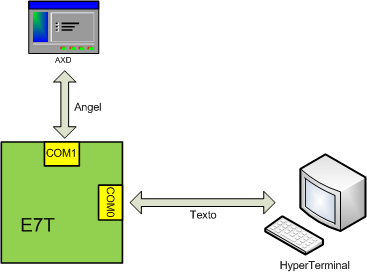
\includegraphics[height=8cm]{figuras/e7t_comm.png}
\caption{Comunica��o da Evaluator-7T em cada porta serial.\label{e7t_comm}}
\end{figure}

% Configuracao e comunicacao da COM0